\chapter{Diseño e Implementación}

En este capítulo mostraremos los detalles del diseño e implementación de diferentes partes del juego.

\section{Gramáticas y frases}

La parte correspondiente a la definición de gramáticas y generación automática de frases es la más relevante del proyecto y lo que la diferencia del resto de juegos de similares características. Por ello consideramos esencial explicar su funcionamiento.

\begin{figure}
    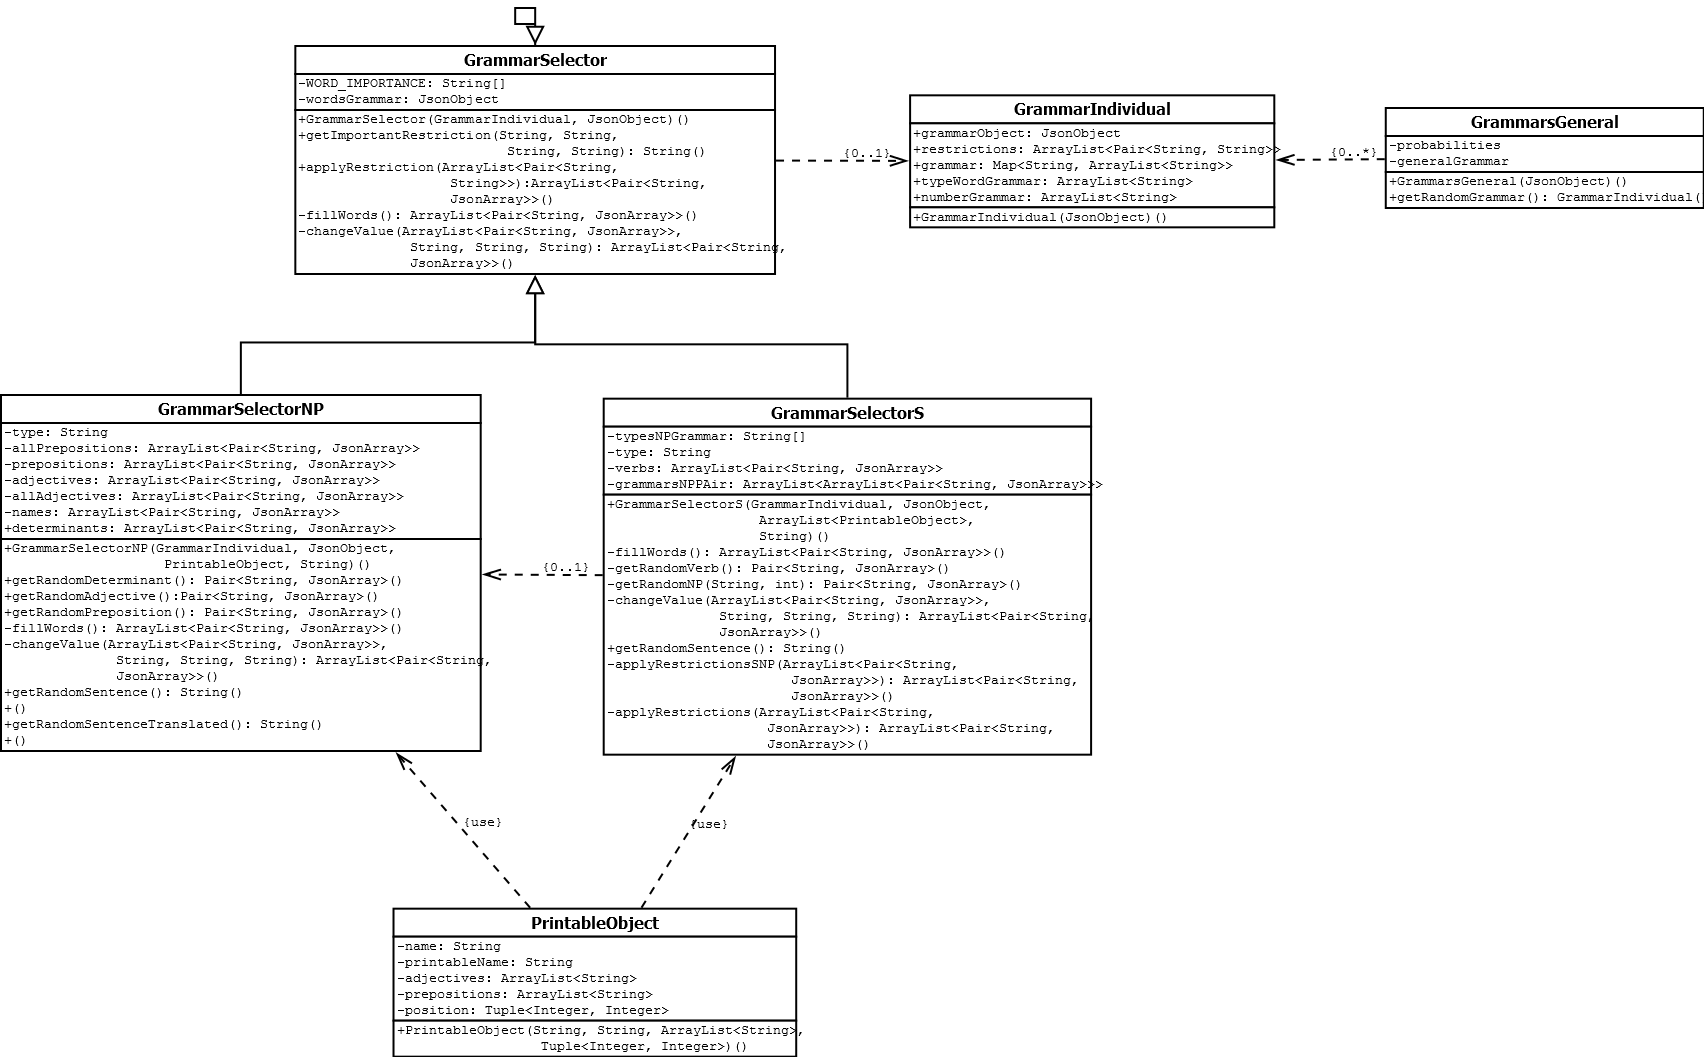
\includegraphics[width=1.5\textwidth,height=1.5\textheight,keepaspectratio,angle=90]{./img/grammarDiagram.png}
  \caption{Diagrama de clases de las gramáticas}
  \label{fig:clasesgramaticas}
\end{figure}

Tal y como se muestra en la Figura ~\ref{fig:clasesgramaticas}, la parte esencial de este módulo consta de seis clases, cuyo funcionamiento detallamos a continuación.

\subsection{Explicación general del funcionamiento}

Tenemos dos clases (\texttt{GrammarSelectorS} y \texttt{GrammarSelectorNP}) que se encargan de generar las frases en base al nombre o nombres sobre los que queremos obtener información. Esta frase se generará en base a gramáticas y diccionarios dados. La clase \texttt{GrammarSelectorNP} crea sintagmas nominales mientras que \texttt{GrammarSelectorS} crea, a su vez, frases usando dichos sintagmas nominales. Ambas usan diccionarios y gramáticas para el idioma concreto especificado en el archivo de configuración \textit{language.properties} (inglés en este caso):

\begin{verbatim}
language=EN
\end{verbatim}

\noindent Parte de la dificultad de generar estas frases está en que los elementos de la misma deben ser congruentes entre sí en base a las restricciones del idioma en cuestión. Por ejemplo, en el caso del español, los nombres, adjetivos y determinantes de una frase nominal deben coincidir en género y número, mientras que en inglés el género no es tenido en cuenta y, en el caso de los adjetivos, tampoco el número. Este tipo de restricciones vienen dadas por las gramáticas, que están especificadas en archivos JSON y que se comentarán más adelante.

Una vez detectemos que dos de las palabras no coinciden, cambiaremos la flexión de la palabra de en base al tipo de la incongruencia (género o número). Por ejemplo, un adjetivo o determinante respecto a un sustantivo.

\begin{lstlisting}[language=java]

if (toChange.equals(value1)) {
    changeToValue = JSONParsing.getElement(restrictions1, type + "opposite");
    typeChangeToValue = typeFirstRestriction; 
     
} else {
    changeToValue = JSONParsing.getElement(restrictions2, type + "opposite");
    typeChangeToValue = typeSecondRestriction;
}
this.changeValue(sentenceArray, toChange, changeToValue, typeChangeToValue);

\end{lstlisting}

\noindent De esta manera, siempre que haya una discordancia entre algunos de los contribuyentes de una frase, iteraremos entre sus elementos ella buscando una solución hasta que sea coherente, cambiando sucesivamente la flexión de las palabras de menos rango dentro de dicha frase para que se adapten al resto.

La clase \texttt{GeneralGrammar}, por su parte, obtiene la información de varias gramáticas, ya que es así como vienen dadas en el fichero, puesto que para describir una misma situación puede haber varias gramáticas aplicables válidas, lo que concuerda con el concepto de \emph{variedad lingüística} del lenguaje humano, es decir, cómo nuestro concepto permite expresar una misma idea o mensaje de diferentes formas. Por ejemplo, ``el héroe ataca al dragón'' y ``él se lanza contra el dragón con la espada mágica''. 
Para ello la clase \texttt{GeneralGrammar}, dispone de una función que devuelve una gramática individual (de la clase \texttt{GrammarIndividual}) de todas las disponibles para cierto caso y es la que usaremos a la hora de generar la frase en sí. Es decir, cuando queremos generar una frase para describir una situación en concreto (por ejemplo cuando un personaje ataca a otro), seleccionaremos una de las gramáticas de todas las que estén disponibles para este tipo de encuentros en el idioma actual (esto lo realiza la clase \texttt{GrammarsGeneral}) y luego usamos esa gramática en particular (clase \texttt{GrammarIndividual}). De esta forma no siempre usaremos la misma para describir un mismo evento (o similar), aumentando la expresividad del sistema y evitando así resultar cargantes.

La clase \texttt{PrintableObject} es una superclase abstracta de la que heredan todos los objetos que pueden ser representados en el juego. Esta clase se encarga de obligar que dichos objetos tengan ciertas variables como el nombre o la capacidad de traducir su nombre a diferentes idiomas, así como una función que devuelve la posición en la que se encuentra en base al usuario y que emplearemos a la hora de describir lo que hay alrededor del personaje.

\subsection{\textit{Input} de gramáticas y diccionario}

Tanto las gramáticas como los diccionarios empleados por el sistema son almacenados como ficheros JSON que el usuario puede modificar o intercambiar, lo que afectará al resultado de las frases generadas.

El sistema requiere tres archivos de entrada para un idioma dado, dos correspondientes a las gramáticas y el tercero correspondiente al diccionario. En el caso de las gramáticas, uno es empleado para generar los sintagmas nominales, mientras que con el otro generamos expresiones más complejas, en su mayor parte a partir de estos sintagmas nominales.

\subsubsection{Gramáticas: Sintagmas nominales}

A continuación mostramos un ejemplo de gramática generadora de sintagma nominal en inglés correspondiente a una estructura DETERMINANTE + ADJETIVO + NOMBRE:

\begin{lstlisting}[style=json]
"DETADJN": {
    "GM_1": {
        "S": 
            [
            {"DET_1": ""}, 
            {"ADJ_1": ""}, 
            {"N_1": ""}
        ],
        "restrictions": [
            {"DET_1.num": "N_1.num"},
            {"N_1.num": "ADJ_1.num"}
        ]
    }
}
\end{lstlisting}

\noindent En estas gramáticas especificamos, primero, el nombre del grupo de gramáticas (en este caso, \texttt{DETADJN}). Este identificador es usado por el programa y ayudará al traductor del sistema a entender el tipo que son.

El siguiente identificador es el nombre de la gramática en particular. Éste no es empleado en el programa, pero su uso es necesario para poder definir varias de ellas sobre el mismo árbol. Por ejemplo, si queremos más gramáticas de tipo \texttt{DETADJN}, necesitaremos que se especifique un nombre para cada una de ellas.

A continuación viene la definición de la gramática en sí. Primero nos encontramos con el apartado \texttt{S}, que es donde se almacenará su definición; y luego el apartado \texttt{restrictions} que, como su nombre indica, es donde especificaremos las restricciones aplicables al anterior.

En el caso de nuestro ejemplo, en la parte de la gramática tenemos, en este caso, \texttt{DET\_1}, que es el primer determinante (y único) de la gramática; \texttt{ADJ\_1}, el primer y único adjetivo que tiene dicha gramática y \texttt{N\_1}, que es el nombre o sustantivo.
En las restricciones detallamos las partes que tienen que coincidir. En este caso solamente tenemos que el determinante, nombre y adjetivo tienen que ser iguales (congruentes) en número. Es decir, que ``the red swords'' no sería generada, sino que generaría ``the red sword''.

Este primer era para inglés, cuyas restricciones son más sencillas que en otros idiomas como el español o el gallego, donde los nombres, determinantes y adjetivos no solamente tienen que coincidir en número, sino también en género. De este modo, la gramática equivalente para el español (y también gallego) sería la siguiente:

\begin{lstlisting}[style=json]
"DETADJN": {
    "GM_1": {
        "S": 
            [
            {"DET_1": ""},
            {"N_1": ""},
            {"ADJ_1": ""}
        ],
        "restrictions": [
            {"DET_1.num": "N_1.num"},
            {"N_1.num": "ADJ_1.num"},
            {"DET_1.gen": "N_1.gen"},
            {"N_1.gen": "ADJ_1.gen"}
        ]
    }
}
\end{lstlisting}

\noindent Nótese que no solamente hemos añadido el género a las restricciones (para que no podamos generar frases como ``la espada rojo'' o ``el espada roja''), sino que también hemos cambiado el orden del nombre y del adjetivo para que correspondan a la estructura típica en español (y gallego). 

A la hora de cambiar la flexión de las palabras que componen la frase dispondremos de un array donde ordenar las palabras por rango de importancia. Un sustantivo es más importante, o tiene mayor rango que un determinante en cuanto a que el sustantivo, como núcleo de la frase nominal, es el que determina el género y número del sintagma con el que deben de coincidir determinantes y adjetivos. De este modo, si alguna de las restricciones no se cumple entre de estos dos elementos, el determinante será el que cambiará para adaptarse al género y número del nombre.

De esta manera podremos adaptar las gramáticas a diferentes idiomas de una forma sencilla y sin necesidad de tocar nada de código.

\subsubsection{Gramáticas: Estructuras complejas}

Las gramáticas para la generación de este tipo de estructuras también pueden hacer a su vez uso de aquellas gramáticas de sintagmas nominales. En este caso, a modo de ejemplo mostramos una gramática correspondiente a la descripción (sencilla) de un ataque: 

\begin{lstlisting}[style=json]
"ATTACK": {
	"S1": {
	    "S": [
	        {"DETADJN_1": ""},
	        {"V_1": ""},
	        {"DETADJN_2": ""},
	        {"SIMPLEPREP_1": ""}
	    ],
	    "restrictions": [
	        {"DETADJN_1.num": "V_1.num"}
	    ]
	},
	"S2": {
	    "S": [
	        {"GENERAL_1": ""},
	        {"V_1": ""},
	        {"SIMPLE_2": ""},
	        {"SIMPLEPREP_1": ""}
	    ],
	    "restrictions": [
	        {"GENERAL_1.num": "V_1.num"}
	    ]
	}
}
\end{lstlisting}

\noindent La estructura de esta gramática es la ya mencionada anteriormente. En este caso vemos que dentro de \texttt{ATTACK} disponemos de dos gramáticas distintas (éste es solamente un ejemplo, en el juego tenemos muchas más disponibles) y éstas llaman a sintagmas nominales como el anterior.
Con la primera gramática podríamos generar una frase del estilo ``The mighty dragon attacks the brave hero with the sword''. En este ejemplo cabe destacar que las restricciones se pueden definir no solamente entre palabras, pero también entre sintagmas nominales (siempre y cuando sea en comparación con una palabra que pueda ser cambiante, en este caso el verbo) y que los sintagmas nominales que son creados dentro de esta gramática tienen sus propias restricciones, por lo que siempre serán generadas de manera correcta.

\subsubsection{Diccionarios}

Al igual que las gramáticas, los diccionarios también están divididos por idiomas y son archivos JSON. Éste es un ejemplo de parte de un diccionario para inglés:

\begin{lstlisting}[style=json]
"DET": {
    "the": [
        {"num": ""},
        {"translation": "the"},
        {"numopposite": "the"},
        {"genopposite": ""}
        {"gender": ""}
    ]
},
\end{lstlisting}

El primer elemento, \texttt{DET}, especifica el tipo de palabra que es (determinante). El siguiente elemento especifica la palabra en sí (\texttt{the}). El resto de elementos estarán en un array de pares (CLAVE, VALOR), aunque en este caso no importa el orden. La clave del primer elemento en esta lista es \texttt{num} correspondiendo al número del término en cuestión, es decir, si el elemento es singular o plural (para esta palabra esta información es innecesaria, por eso es un string vacío) mientras que en \texttt{numopposite} guardaremos la flexión de la palabra en el número contrario (si la palabra es singular, entonces guardaremos la palabra en plural).
El segundo es \texttt{translation}. Todas las palabras entre los diccionarios serán las mismas o, por lo menos, las que están definidas en inglés también deben estarlo en otros idiomas. En este valor almacenaremos la traducción de esta palabra al idioma del diccionario que estaremos definiendo.
Los elementos \texttt{gender} y \texttt{genopposite}, al igual que con \texttt{num} y \texttt{numopposite}, almacenan el género de la palabra y la palabra de género contrario.

Retomando nuestro ejemplo anterior, con los determinantes en inglés no hay mucho cambio, pero en español sí que es bastante diferente:

\begin{lstlisting}[style=json]
"DET": {
        "el": [
            {"num": "sing"},
            {"translation": "el"},
            {"numopposite": "los"},
            {"genopposite": "la"},
            {"gen": "mas"}
        ],
        "la": [
            {"num": "sing"},
            {"translation": "la"},
            {"numopposite": "las"},
            {"genopposite": "the"},
            {"gen": "fem"}
        ],
        "los": [
            {"num": "plural"},
            {"translation": "los"},
            {"numopposite": "the"},
            {"genopposite": "las"},
            {"gen": "mas"}
        ],
        "las": [
            {"num": "plural"},
            {"translation": "las"},
            {"numopposite": "la"},
            {"genopposite": "los"},
            {"gen": "fem"}
        ]
    },
\end{lstlisting}

\noindent En este caso vemos que \texttt{numopposite} y \texttt{genopposite} apuntan ahora a \texttt{la} y \texttt{los}, que corresponden a la flexión en número y género, respectivamente. De esta forma  obtendremos el término que queramos siempre y cuando el programa precise obtener un tipo de palabra concreta en base a las restricciones que contenga la gramática.

\section{Otras partes del sistema}

Las gramáticas juegan un papel muy importante en el proyecto, pero hay otras partes relevantes del sistema que merecen una atención especial. Aquí mencionamos las más importantes:

\subsection{Interfaz de usuario para el texto generado}

Para que nuestro sistema pueda aprovecharse del software de lectura de pantalla empleado por usuarios invidentes, no basta simplemente con que saque el texto por pantalla. Debe de hacerse de forma que el software de lectura pueda leerlo, lo que no es del todo trivial dado que hay que tener en cuenta diferentes aspectos para que el lector lea lo que queramos y no otras partes que no nos interesan. Más información sobre este tema se encuentra disponible en el Apéndice ~\ref{ref:instalacion} de esta memoria.

\subsubsection{Primer planteamiento: \textit{pop-ups}}

La forma más sencilla de mostrar este texto es mostrar un \emph{pop-up} cada vez que una frase es generada. De esta forma el usuario se enterará inmediatamente de lo que está sucediendo y, en caso de que haya una persona vidente a su lado, ésta también podrá leer la frase que se ha generado. Además, la frase no desaparecerá hasta que se presione la tecla de \textit{intro} o se haga click en \textit{Aceptar}, por lo que es muy sencillo reproducirla la cantidad de veces que se desee.

La Figura ~\ref{fig:lastiterationui} muestra un ejemplo de uso sencillo para esta implementación.

\begin{figure}
    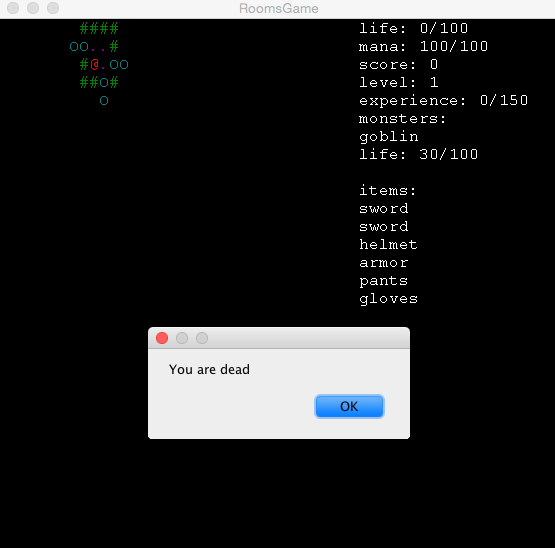
\includegraphics[width=\textwidth,height=\textheight,keepaspectratio]{./img/firstiterationui.png}
  \caption{Versión preliminar de la interfaz de usuario para el texto generado basada en el uso de \textit{pop-ups}}
  \label{fig:firstiterationui}
\end{figure}

\subsubsection{Segundo planteamiento: \textit{TextArea}}

En base al \textit{feedback} recibido decidimos abandonar esta prima solución por tres razones. La primera es que resulta desconcertante para el jugador vidente, dado que, en su caso, no es necesario. Esto se podría solventar añadiendo una opción que permita activar o desactivar esta función, aunque no es la mejor solución para este problema.
La segunda razón es que estos \textit{pop-ups} no son un mecanismo óptimo para mostrar salidas rutinarias, como en nuestro caso, pues rompe el ``flujo de trabajo''.
La tercera y última razón es que los usuarios invidentes no suelen hacer uso de elementos de este tipo, sino que están más acostumbrados a emplear áreas de texto donde se almacenan las últimas frases generadas por el programa en cuestión.

En base a estas ideas decidimos crear un área de texto que permanecerá abierta siempre y cuando el jugador no decida cerrarla, (permitiendo a los usuarios videntes prescindir de ella). En el momento en que sucede algo en el juego que requiere generar una descripción, dicha descripción será enviada al área de texto, el ``foco'' de las aplicaciones cambiará para que se sitúe en esa ventana y el lector de pantalla que estamos usando leerá dicha descripción. Mientras generemos frases el ``foco'' seguirá en ese área de texto, si bien las teclas que pulsemos seguirán actuando sobre el juego para evitar romper el flujo de trabajo). El foco solamente volverá al juego cuando pulsemos una tecla que no genere una nueva frase.
De esta forma solucionamos todos los inconvenientes que los \textit{pop-ups} causaban a los usuarios, mejorando la interfaz gráfica y la accesibilidad del proyecto.

En la Figura ~\ref{fig:lastiterationui} se puede encontrar una captura de pantalla donde se muestra un ejemplo de uso para esta nueva implementación.

\begin{figure}
    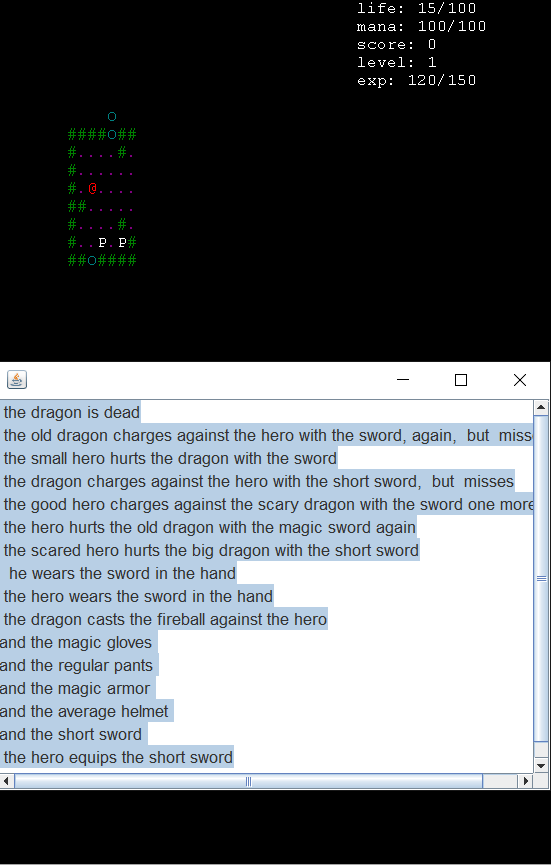
\includegraphics[width=\textwidth,height=\textheight,keepaspectratio]{./img/lastiterationui.png}
  \caption{Versión definitiva de la interfaz de usuario para el texto generado basada en el uso de una \textit{TextArea}}
  \label{fig:lastiterationui}
\end{figure}

\subsection{Generación aleatoria de mapas y elementos}

Como ya se indicó en la Sección ~\ref{game:roguelikeis}, la generación aleatoria de los mapas y de los elementos dentro de los mismos es una de las características que un juego de género \textit{roguelike}. A continuación explicaremos las decisiones tomadas a este respecto.

A la hora de generar el mapa en sí tenemos en cuenta tres elementos fundamentales: mapas, habitaciones y puertas. Cada mapa generado consta de un conjunto de habitaciones (que vienen limitadas por sus propias paredes), cuyo tamaño y forma cambia de manera aleatoria. Cada puerta une dos habitaciones, asegurándonos que ninguna de las estancias queda sin la posibilidad de ser alcanzable por el jugador. También se han introducido columnas que se encuentran dentro de cada habitación para que tanto el jugador que controla el usuario como los enemigos tengan que esquivarlas y puedan usarlas en su favor en los combates. Hay que tener en cuenta que ningún personaje puede moverse a una posición donde se encuentra una columna por lo que, a la hora de generarlas, se comprueba que no bloquean el acceso a la puerta o, si lo hacen, que haya otra entrada por la que se pueda acceder a dicha estancia.

\subsubsection{Primer planteamiento: Generación completamente aleatoria}

En un primer momento nuestra decisión fue la de generar todo de manera aleatoria, sin considerar ningún aspecto externo, pero manteniendo la generalidad en el código para poder cambiar su comportamiento en cualquier momento. Esto causaba que algunas mazmorras fueran muy complicadas cuando el jugador todavía no tenía el equipamiento necesario para enfrentarse a dichos enemigos o demasiado sencilla en otros momentos.

Este problema fue mencionado la primera vez que recibimos \textit{feedback} y por ello decidimos cambiarlo por algo un poco más complejo.

\subsubsection{Segunda idea: Generador de encuentros}
\label{generadorencuentros}

En el mundo del rol, tener en cuenta ciertas características del usuario para generar elementos externos se denomina \textit{generación de encuentros}. De este modo, en vez de generar mapas, enemigos y elementos de manera completamente aleatoria, podemos generarlos en base al nivel que tienen ciertos personajes. Si el personaje que controla el usuario tiene nivel 10, entonces los adversarios que se encuentren deberían ser de un nivel similar, por ejemplo entre 8 y 12 y así mantener un nivel de dificultad equilibrado, no demasiado fácil ni demasiado difícil, envitando que el jugador caiga en el tedio o en la frustración. De forma similar, los elementos que dichos oponentes suelten al morir, tales como espadas y armaduras, también deberían tener un nivel similar para que la progresión tenga sentido y eliminar enemigos implique un cierto nivel de recompensa.

De esta forma, en base al nivel dado, podremos generar contrincantes con diferentes características que se adapten a lo que necesitamos. Mostramos un ejemplo cómo generar un enemigo en una habitación en concreto:

\begin{lstlisting}[language=java]
Rat rat = new Rat(this.getMap(), this, position, new ArrayList<String>(), level);
\end{lstlisting}

\subsection{Comportamiento de los enemigos}
\label{sec:ia}

Como cabe suponer, los adversarios que nos encontramos en el juego se moverán de diferentes formas, por lo que tendremos que diseñarlo de una manera genérica que nos permita realizar esto de la forma más simple posible.
Para ello nos hemos basado en el patrón de diseño \textit{estrategia} porque se adapta perfectamente a nuestros requisitos.

Los tipos de movimiento que tenemos disponibles en el juego actualmente de cara a los enemigos son los siguientes:

\paragraph{RandomMovement:} Los enemigos son ``pasivos'', es decir, no atacarán a ningún personaje ni tampoco irán hacia él en ningún momento.

\paragraph{FollowingMovementDumb:} Los contrincantes que tengan este tipo de comportamiento son más ``agresivos''. Seguirán al jugador e intentarán atacarle, pero no se mueven de una forma óptima para lograr su meta, por lo que esquivarlos no suele ser muy complicado.

\paragraph{FollowingMovement:} Este tipo de comportamiento es el más complejo y ``agresivo''. El enemigo se moverá de manera precisa para llegar lo antes posible al usuario y usará todo tipo de tácticas para derrotarlo, tales como el uso de magia o atacándole cuerpo a cuerpo.

\noindent Gracias a nuestro diseño, crear nuevos tipos de comportamientos es una tarea trivial, ya que solamente tendríamos que implementar la interfaz \textit{Movement} con la única función que posee e insertar en él el código del nuevo tipo de movimiento.

La Figura ~\ref{fig:iaenemy} mostramos el diagrama de clases que hemos implementado en nuestro sistema y que contiene el patrón de diseño \textit{estrategia}, tal y como hemos comentado.

\begin{figure}
    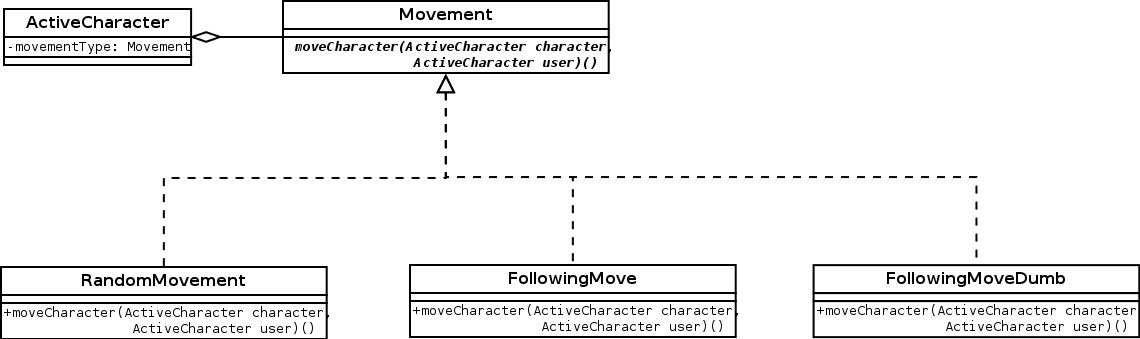
\includegraphics[width=\textwidth,height=\textheight,keepaspectratio]{./img/iaenemy.png}
  \caption{Diagrama de clases para el comportamiento de los enemigos}
  \label{fig:iaenemy}
\end{figure}

\subsection{Interacción entre objetos, personajes y hechizos}

La Figura ~\ref{fig:charactersitems} muestra las relaciones entre las clases abstractas e interfaces de los objetos, personajes, movimientos y hechizos de nuestro juego.

La clase \texttt{Character} contiene la información básica de los personajes, mientras que en \texttt{ActiveCharacter} se encuentra información adicional que posibilita que el personaje se mueva en base a una clase que implemente la interfaz \texttt{Movement} e interactúe con el resto de elementos del juego, por lo que es la clase de la que todos los enemigos heredan. Esto ayuda a que en un futuro puedan crearse personajes como vendedores que no necesiten moverse de manera sencilla. 
Todos los personajes pueden tener \texttt{Items}, que son consumibles (pociones) o elementos que el jugador puede equipar (espadas, cascos, botas, etc.). Sin embargo, éstos no tienen por qué pertenecer a ningún personaje, se pueden encontrar en el mapa para que el personaje que el jugador controla pueda cogerlos.
Por último, un personaje en concreto también puede tener diferente número de hechizos, representados en el diagrama por la clase abstracta \texttt{Spell}, que harán daño en cierta área y que también costarán maná. De la misma manera que con las clases \texttt{Movement} o \texttt{ActiveCharacter}, extenderla para crear nuevos hechizos es muy sencillo, lo que permite que los elementos primordiales del juego sean fácilmente extendibles.

\begin{figure}
    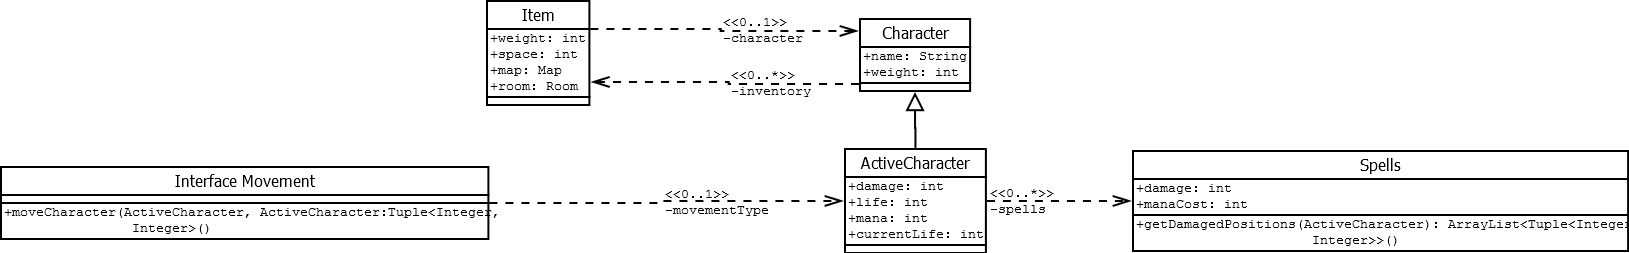
\includegraphics[width=\textwidth,height=0.15\textwidth]{./img/charactersitems.png}
	\caption{Diagrama de clases abstractas e interfaces sobre los objetos, personajes, hechizos y movimiento}
	\label{fig:charactersitems}
\end{figure}

\section{Herramientas empleadas}

En esta sección hablaremos sobre las tecnologías y herramientas empleadas en este proyecto y, si cabe, las razones por la que fueron elegidas. En primer lugar describiremos las herramientas y bibliotecas que hemos usado y, en segundo lugar, las herramientas de comunicación con usuarios y \textit{testers}.

\subsection{Herramientas software empleadas}

\paragraph{Java:} Este lenguaje de programación orientado a objetos es uno de los lenguajes de programación más utilizados en la industria. Una de sus principales características es que es multiplataforma, es decir, puede ser ejecutado en cualquier sistema operativo que tenga la \textit{Java Virtual Machine} instalada sin necesidad de realizar cambios en el código (WORA, \textit{``Write once, run anywhere''}). Esta característica es primordial en nuestro caso, dado que nuestros usuarios potenciales usan gran variedad de sistemas operativos, mayor incluso que respecto al usuario estándard	.

 \paragraph{Eclipse:}\footnote{\url{https://eclipse.org}} Es un IDE (entorno de desarrollo integrado) usado para escribir código en múltiples lenguajes. También incluye una serie de \textit{plugins} que facilitan y automatizan muchas de las labores a realizar, tales como el uso de sistema de controles, ejecución de código y tests, herramientas de \textit{debug}, autocompletado de código, etc.

 \paragraph{Git:}\footnote{\url{https://goo.gl/IKsKt5}} Sistema de control de versiones distribuido. Es el control de versiones referencia en la mayoría de empresas y proyectos de software libre gracias a su rapidez y, al ser distribuido, permite trabajar y realizar \textit{commits} del código sin necesidad de conexión a Internet.

 \paragraph{GitHub:}\footnote{\url{github.com}} Plataforma de desarrollo colaborativo usada para alojar proyectos usando el sistema de control de versiones Git. La mayoría de proyectos de código abierto lo usan, dado que es gratuito, aunque permite la opción de almacenar el código de forma privada previo pago.

\paragraph{JSON:} \textit{JavaScript Object Notation}. Es un formato muy usado en APIs para intercambio de datos, similar a XML. En nuestro caso lo usamos para definir las gramáticas y diccionarios de nuestro proyecto, dado que es muy sencillo de leer y especificar.

\paragraph{\textit{NVDA}:}\footnote{\url{www.nvaccess.org}} Lector de pantalla de código libre para Windows que lee el tipo de ventanas y texto que se encuentran en la pantalla, facilitando el uso del ordenador y otros dispositivos a los usuarios invidentes. 
Orca\footnote{\url{https://goo.gl/nW9UaZ}} es, en cierta medida, su equivalente en Linux. Otras alternativas son BrowseAloud\footnote{\url{https://goo.gl/GoghW7}} o Microsoft Narrator\footnote{\url{http://goo.gl/OAB7VC}}. Hemos elegido \textit{NVDA} por ser la alternativa libre más usada por este tipo de usuarios.

\paragraph{\textit{Gson}:}\footnote{\url{https://goo.gl/zPCXen}} Hay numerosas bibliotecas que nos permiten analizar y trabajar con este formato en Java. En nuestro caso hemos usado \href{https://goo.gl/zPCXen}{\textit{Gson}} para transformar archivos JSON a objetos de Java y viceversa.

\paragraph{JCurses:}\footnote{\url{https://github.com/sunhong/jcurses}} \textit{The Java Curses Library} es una biblioteca para el desarrollo de aplicaciones de terminal para JAVA. Es similar a AWT,\footnote{\textit{Abstract Window Toolkit.} Kit de herramientas de interfaz de usuario de la plataforma original de Java} pero basada en el sistema de ventanas \textit{Curses} de \textit{UNIX}.

\paragraph{Libjcsi:}\footnote{\url{www.slashie.net/libjcsi}} Biblioteca de representación gráfica que trabaja sobre JCurses y simplifica la tarea de representar y refrescar elementos del terminal.

\subsection{Herramientas de comunicación con usuarios y \textit{testers}}

\paragraph{Listas de Correo:} Las listas de correo son un método de comunicación muy usado por diferentes comunidades, especialmente en el desarrollo de software, que ayudan a los usuarios que participan en ellas a enviar correos a múltiples personas que lo deseen de forma anónima y, al mismo tiempo, tener un historial de las respuestas devueltas por los mismos. En nuestro caso las hemos usado para comunicarnos con un grupo de usuarios y desarrolladores de videojuegos para invidentes\footnote{\url{tiflo-juegos@googlegroups.com}} y recibir \textit{feedback} por parte de la comunidad.

 \paragraph{Reddit:}\footnote{\url{www.reddit.com}} Web creada en 2005 y que actualmente se encuentra en el top 50 de las más visitadas del mundo. Cuenta con una comunidad gigante que está dividida en muchísimos subgrupos dependiendo del tema a tratar. La hemos usado como una herramienta de \textit{feedback}. Especialmente los \textit{subreddits} de \href{https://www.reddit.com/r/ColorBlind/}{daltónicos}, de \href{https://www.reddit.com/r/blind/}{personas que sufren de ceguera}, \href{https://www.reddit.com/r/gamedev/}{desarrolladores de videojuegos} y \href{https://www.reddit.com/r/roguelikes/}{roguelikes}.
